\nte[Section 1.2]{Sep 28 2023 Wed (14:01:51)}{Row Reduction and Echelon Forms}

This lecture redefines the method of
\cref{sec:solving_linear_systems_with_row_operations} into a row reduction
algorithm that will enable us to analyze any matrix. By using only the first
part of this algorithm, we will be able to answer the fundamental existence and
uniqueness questions.

\begin{definition}[Echelon Form]
  \label{def:echelon_form}

  A matrix is an \textbf{echelon form} if it has the following properties:
  \begin{enumerate}
    \label{enum:echlon_form}

    \item All nonzero rows are above any rows of all zeros.
    \item Each leading entry of a row is in a column to the right of the leading
      entry of the row above it.
    \item All entries in a column below a leading entry are zeros.
  \end{enumerate}
\end{definition}

\begin{note}
  \label{nte:nonzero_rows}

  A nonzero row is a row with at least one nonzero entry.
\end{note}

\begin{example}
  \label{exm:echelon_form}

  Below are some examples of matrices in echelon form.

  \begin{minipage}{.5\linewidth}
    \[%
      \begin{bNiceArray}{ccc|c}[columns-width=auto]
        \circled{2} & -1 & 0 & 1 \\
        0 & \circled{2} & 3 & -2 \\
        0 & 0 & 0 & 0
      \end{bNiceArray}
    .\]%
  \end{minipage}
  \begin{minipage}{.5\linewidth}
    \[%
      \begin{bNiceArray}{cccccc|c}[columns-width=auto]
        0 & \circled{7} & 3 & 0 & -1 & 1 & -2 \\
        0 & 0 & 0 & \circled{3} & 1 & 4 & 0 \\
        0 & 0 & 0 & 0 & \circled{3} & 0 & -3 \\
        0 & 0 & 0 & 0 & 0 & 0 & 0 \\
      \end{bNiceArray}
    .\]%
  \end{minipage}
\end{example}

\begin{definition}[Reduced Echelon Form]
  \label{def:reduced_echelon_form}

  If a matrix in echelon form satisfies the following additional conditions,
  then it is in \textbf{reduced echelon form}:
  \begin{enumerate}
    \label{enum:reduced_echelon_form}

    \item The leading entry in each nonzero row is $1$.
    \item Each leading $1$ is the only nonzero entry in its column.
  \end{enumerate}
\end{definition}

\begin{example}
  \label{exm:reduced_echelon_form}

  Below are some examples of matrices in reduced echelon form.

  \begin{minipage}{.5\linewidth}
    \[%
      \begin{bNiceArray}{ccc|c}[columns-width=auto]
        \circled{1} & 0 & 5 & 1 \\
        0 & \circled{1} & -1 & 3 \\
        0 & 0 & 0 & 0 \\
      \end{bNiceArray}
    .\]%
  \end{minipage}
  \begin{minipage}{.5\linewidth}
    \[%
      \begin{bNiceArray}{cccccc|c}[columns-width=auto]
        0 & \circled{1} & -6 & 0 & 0 & 1 & -2 \\
        0 & 0 & 0 & \circled{1} & 0 & 5 & 3 \\
        0 & 0 & 0 & 0 & \circled{1} & -1 & 2 \\
        0 & 0 & 0 & 0 & 0 & 0 & 0 \\
      \end{bNiceArray}
    .\]%
  \end{minipage}
\end{example}

\begin{theorem}[Uniqueness of the Reduced Echelon Form]
  \label{thm:uniqueness_of_the_reduced_echelon_form}

  Each $m \times n$ matrix $A$ is row equivalent to a unique reduced echelon
  matrix $U$.
\end{theorem}

\begin{proof}
  \label{prf:uniqueness_of_the_reduced_echelon_form}

  The row reduction algorithm shows that there exists at least one such matrix
  $U$. Suppose that $A$ is row equivalent to matrices $U$ and $V$ in reduced
  echelon form. The leftmost nonzero entry in a row of $U$ is a ``leading $1$.''
  Call the location of such a leading $1$ a pivot position, and call the column
  that contains it a pivot column. (This definition uses only the echelon nature
  of $U$ and $V$ and does not assume the uniqueness of the reduced echelon
  form.)

  The pivot columns of $U$ and $V$ are precisely the nonzero columns that are
  not linearly dependent on the columns to their left. (This condition is
  satisfied automatically by a first column if it is nonzero.) Since $U$ and $V$
  are row equivalent (both being row equivalent to $A$), their columns have the
  same linear dependence relations. Hence, the pivot columns of $U$ and $V$
  appear in the same locations. If there are $r$ such columns, then since $U$
  and $V$ are in reduced echelon form, their pivot columns are the first $r$
  columns of the $m \times n$ identity matrix. Thus, corresponding pivot columns
  of $U$ and $V$ are equal.

  Finally, consider any nonpivot column of $U$, say column $j$. This column is
  either zero or a linear combination of the pivot columns to its left (because
  those pivot columns are a basis for the space spanned by the columns to the
  left of column $j$). Either case can be expressed by writing $U\x = \zero$ for
  some $\x$ whose $j$th entry is $1$. Then $V\x = \zero$, too, which says that
  column $j$ of $V$ is either zero or the same linear combination of the pivot
  columns of $V$ to its left. Since corresponding pivot columns of $U$ and $V$
  are equal, columns $j$ of $U$ and $V$ are also equal. This holds for all
  nonpivot columns, so $V = U$, which proves that $U$ is unique.
\end{proof}

\section{Pivot Position}
\label{sec:pivot_position}

When row operations on a matrix produce an echelon form, further row operations
to obtain the reduced echelon form do not change the positions of the leading
entries. Since the reduced echelon form is unique, the leading entries are
always in the same positions in any echelon form obtained from a given matrix.

\begin{definition}[Pivot Position]
  \label{def:pivot_position}

  A \textbf{pivot position} in a matrix is the location of a leading entry in
  its echelon form.

  A \textbf{pivot column} is a column which contains a pivot position.

  A \textbf{pivot} itself is a nonzero number of an echelon form of located
  in a pivot position
\end{definition}

\begin{note}
  \label{nte:pivot_position}

  All pivot positions will be circled.
\end{note}

\begin{question}
  \label{qst:pivot_position}

  Row reduce the matrix below to echelon form, and locate the pivot columns.
  \[%
    \begin{bNiceArray}{cccc|c}[columns-width=auto]
      0 & -3 & -6 & 4 & 9 \\
      -1 & -2 & -1 & 3 & 1 \\
      -2 & -3 & 0 & 3 & -1 \\
      1 & 4 & 5 & -9 & -7 \\
    \end{bNiceArray}
  .\]%
\end{question}

\begin{solution}
  \label{sol:pivot_position}

  The pivot columns are the columns containing the pivot positions.

  A nonzero entry must be placed at the top left corner of the matrix. That's
  why it's reasonable to switch the first and last rows, since that will make
  the mental computation easier.
  \[%
    \sysdelim..\systeme*{
      R_1 \rightarrow R_4
    } \longleftrightarrow
    \begin{bNiceArray}{cccc|c}[columns-width=auto]
      \circled{1} & 4 & 5 & -9 & -7 \\
      -1 & -2 & -1 & 3 & 1 \\
      -2 & -3 & 0 & 3 & -1 \\
      0 & -3 & -6 & 4 & 9 \\
    \end{bNiceArray}
  .\]%

  Next, we need to create zeros below the first pivot by adding multiples of the
  first row to the rows below.
  \[%
    \sysdelim..\systeme{
      R_1 + R_2 \rightarrow R_2,
      2R_1 + R_3 \rightarrow R_3
    } \longleftrightarrow
    \begin{bNiceArray}{cccc|c}[columns-width=auto]
      \circled{1} & 4 & 5 & -9 & -7 \\
      0 & \circled{2} & 4 & -6 & -6 \\
      0 & 5 & 10 & -15 & -15 \\
      0 & -3 & -6 & 4 & 9 \\
    \end{bNiceArray}
  .\]%

  We can then perform the following row operations to get the final two pivots
  \[%
    \sysdelim..\systeme{
      \-\sfrac{5}{2}R_2 + R_3 \rightarrow R_3,
      \sfrac{3}{2}R_2 + R_4 \rightarrow R_4
    } \longleftrightarrow
    \begin{bNiceArray}{cccc|c}[columns-width=auto]
      \circled{1} & 4 & 5 & -9 & -7 \\
      0 & \circled{2} & 4 & -6 & -6 \\
      0 & 0 & 0 & 0 & 0 \\
      0 & 0 & 0 & -5 & 0 \\
    \end{bNiceArray}
  .\]%

  However, there isn't any way to create a new pivot in column $3$. We can
  interchange the third and fourth rows.
  \[%
    \sysdelim..\systeme*{
      R_3 \rightarrow R_4
    } \longleftrightarrow
    \begin{bNiceArray}{cccc|c}[columns-width=auto]
      \circled{1} & 4 & 5 & -9 & -7 \\
      0 & \circled{2} & 4 & -6 & -6 \\
      0 & 0 & 0 & \circled{-5} & 0 \\
      0 & 0 & 0 & 0 & 0 \\
    \end{bNiceArray}
  .\]%

  This reveals that columns $1$, $2$, and $4$ are pivot columns.
\end{solution}

% section pivot_position (end)

\section{The Row Reduction Algorithm}
\label{sec:the_row_reduction_algorithm}

This algorithm is broken up into two phases.
\begin{enumerate}
  \label{enum:row_reduction_algorithm_phases}

  \item The \textbf{forward phase}, which consists of $4$ steps. Once you
    complete these steps, the matrix will be in echelon form.

  \item The \textbf{backward phase}, which consists of $1$ step. Once you
    complete the step, the matrix will be in reduced echelon form.
\end{enumerate}

\subsection{Forward Phase}
\label{sub_sec:forward_phase}

Here are the $4$ steps of the forward phase.
\begin{enumerate}
  \label{enum:forward_phase_steps}

  \item Begin with the leftmost nonzero column. This will be a pivot column, and
    the top position with be its pivot position.

  \item If the pivot position selected does not have a nonzero entry, switch
    rows so that it does. You want to switch rows so that the pivot is $1$ or
    $-1$.

  \item Use row replacement operations to create zeros in all positions below
    the pivot.

  \item Cover the row containing the pivot position and cover all rows, if any,
    above it. Apply steps $1$ through $3$ to the submatrix that remains. Repeat
    the process until there are no more nonzero rows to modify.
\end{enumerate}

\begin{question}
  \label{qst:forward_phase}

  Use the row reduction algorithm to find the echelon form of the matrix below.
  \[%
    \begin{bNiceArray}{ccc|c}[columns-width=auto]
      0 & 2 & -8 & 8 \\
      1 & -2 & 1 & 0 \\
      5 & 0 & -5 & 10 \\
    \end{bNiceArray}
  .\]%
\end{question}

\begin{solution}
  \label{sol:forward_phase}

  The pivot position must a nonzero element at the top left corner of the
  matrix. Since the top left corner of $A$ is $0$, we need to interchange the
  first row with another row. It doesn't matter which row you choose, but since
  the second row has a $1$ in the first column, we'll interchange the first and
  second rows.
  \[%
    \sysdelim..\systeme*{
      R_1 \rightarrow R_2
    } \longleftrightarrow
    \begin{bNiceArray}{ccc|c}[columns-width=auto]
      \circled{1} & -2 & 1 & 0 \\
      0 & 2 & -8 & 8 \\
      5 & 0 & -5 & 10 \\
    \end{bNiceArray}
  .\]%

  Now we can perform the row operations to create zeros below the pivot.
  \[%
    \sysdelim..\systeme*{
      -5R_1 + R_3 \rightarrow R_3
    } \longleftrightarrow
    \begin{bNiceArray}{ccc|c}[columns-width=auto]
      \circled{1} & -2 & 1 & 0 \\
      0 & \circled{2} & -8 & 8 \\
      0 & 10 & -10 & 10 \\
    \end{bNiceArray}
  .\]%

  Next, we need to create zeros below the second pivot.
  \[%
    \sysdelim..\systeme*{
      -5R_2 + R_3 \rightarrow R_3
    } \longleftrightarrow
    \begin{bNiceArray}{ccc|c}[columns-width=auto]
      \circled{1} & -2 & 1 & 0 \\
      0 & \circled{2} & -8 & 8 \\
      0 & 0 & \circled{30} & -30 \\
    \end{bNiceArray}
  .\qedhere\]%
\end{solution}

% subsection forward_phase (end)

\subsection{Backward Phase}
\label{sub_sec:backward_phase}

The backward phase consists of one step.
\begin{enumerate}
  \label{enum:backward_phase_steps}

  \item Begin with the rightmost pivot. If it is not $1$, then make it into a
    $1$ by row scaling. Then use row replacement to create zeros above this
    pivot. Move to the next pivot to the left and repeat this step until there
    are no more pivots to modify.
\end{enumerate}

\begin{question}
  \label{qst:backward_phase}

  Take the echelon matrix from \cref{sol:forward_phase} and use the
  backward phase of the row reduction algorithm to find the reduced echelon
  form of the matrix.
\end{question}

\begin{solution}
  \label{sol:backward_phase}

  We need to start on the rightmost pivot and do two things.
  \begin{enumerate}
    \label{enum:backward_phase}

    \item Make the pivot $1$.
    \item Create zeros above the pivot.
  \end{enumerate}

  The rightmost pivot is $30$, so we need to make it $1$ by multiplying
  the whole row by $\sfrac{1}{30}$.
  \[%
    \sysdelim..\systeme*{
      \sfrac{1}{30}R_3 \rightarrow R_3
    } \longleftrightarrow
    \begin{bNiceArray}{ccc|c}[columns-width=auto]
      \circled{1} & -2 & 1 & 0 \\
      0 & \circled{2} & -8 & 8 \\
      0 & 0 & \circled{1} & -1 \\
    \end{bNiceArray}
  .\]%
  Now we need to create zeros above the pivot.
  \[%
    \sysdelim..\systeme{
      8R_3 + R_2 \rightarrow R_2,
      \-R_3 + R_1 \rightarrow R_1
    } \longleftrightarrow
    \begin{bNiceArray}{ccc|c}[columns-width=auto]
      \circled{1} & -2 & 0 & 1 \\
      0 & \circled{2} & 0 & 0 \\
      0 & 0 & \circled{1} & -1 \\
    \end{bNiceArray}
  .\]%
  The next pivot is $2$, so we need to make it $1$ by multiplying the whole row
  by $\sfrac{1}{2}$.
  \[%
    \sysdelim..\systeme*{
      \sfrac{1}{2}R_2 \rightarrow R_2
    } \longleftrightarrow
    \begin{bNiceArray}{ccc|c}[columns-width=auto]
      \circled{1} & -2 & 0 & 1 \\
      0 & \circled{1} & 0 & 0 \\
      0 & 0 & \circled{1} & -1 \\
    \end{bNiceArray}
  .\]%
  Lastly, we need to make all the zeros above the second pivot zeros.
  \[%
    \sysdelim..\systeme*{
      2R_2 + R_1 \rightarrow R_1
    } \longleftrightarrow
    \begin{bNiceArray}{ccc|c}
      \circled{1} & 0 & 0 & 1 \\
      0 & \circled{1} & 0 & 0 \\
      0 & 0 & \circled{1} & -1 \\
    \end{bNiceArray}
  .\]%
  Converting them back variables gives us
  \begin{align*}
    x_1 &= 1 \\
    x_2 &= 0 \\
    x_3 &= -1
  ,\end{align*}
  which gives us our final matrix solution, $(1, 0, -1)$.
\end{solution}

\begin{note}
  \label{nte:backward_phase}

  The key things to remember in order to perform the Row Reduction Algorithm
  efficiently is to create zeros below the pivots first (which is the forward
  phase), and then create zeros above the pivots (which is the backwards phase).
\end{note}

% subsection backward_phase (end)

% section the_row_reduction_algorithm (end)

\section{General Solutions of Linear Systems}
\label{sec:general_solutions_of_linear_systems}

\begin{definition}[Basic and Free Variables]
  \label{def:basic_and_free_variables}

  Variables of a linear system are ordered along the columns of its augmented
  matrix. A \textbf{basic variable} is a variable corresponding to a pivot
  column. While variables not corresponding to a pivot column are \textbf{free
  variables}. That is, variables that can be assigned any value.
\end{definition}

\begin{question}
  \label{qst:basic_and_free_variables}

  Solve the following linear system using the Row Reduction Algorithm
  \[%
    \sysdelim..\systeme{
      3x_2 - 6x_3 + 6x_4 + 4x_5 = -5,
      3x_1 - 7x_2 + 8x_3 - 5x_4 + 8x_5 = 9,
      3x_1 - 9x_2 + 12x_3 - 9x_4 + 6x_5 = 15
    }
  .\]%
\end{question}

\begin{solution}
  \label{sol:basic_and_free_variables}

  First, write it out as an augmented matrix
  \[%
    \begin{bNiceArray}{ccccc|c}[columns-width=auto]
      0 & 3 & -6 & 6 & 4 & -5 \\
      3 & -7 & 8 & -5 & 8 & 9 \\
      3 & -9 & 12 & -9 & 6 & 15 \\
    \end{bNiceArray}
  .\]%

  Next, perform the Row Reduction Algorithm
  \begin{align*}
    \sysdelim..\systeme*{
      R_1 \rightarrow R_3
    } &\longleftrightarrow
    \begin{bNiceArray}{ccccc|c}[columns-width=auto]
      \circled{3} & -9 & 12 & -9 & 6 & 15 \\
      3 & -7 & 8 & -5 & 8 & 9 \\
      0 & 3 & -6 & 6 & 4 & -5 \\
    \end{bNiceArray} \\
    \sysdelim..\systeme*{
      \-R_1 + R_2 \rightarrow R_2
    } &\longleftrightarrow
    \begin{bNiceArray}{ccccc|c}[columns-width=auto]
      \circled{3} & -9 & 12 & -9 & 6 & 15 \\
      0 & \circled{2} & -4 & 4 & 2 & 6 \\
      0 & 3 & -6 & 6 & 4 & -5 \\
    \end{bNiceArray} \\
    \sysdelim..\systeme*{
      \-\sfrac{3}{2}R_2 + R_3 \rightarrow R_3
    } &\longleftrightarrow
    \begin{bNiceArray}{ccccc|c}[columns-width=auto]
      \circled{3} & -9 & 12 & -9 & 6 & 15 \\
      0 & \circled{2} & -4 & 4 & 2 & 6 \\
      0 & 0 & 0 & 0 & \circled{1} & 4 \\
    \end{bNiceArray} \\
    \sysdelim..\systeme{
      \-2R_3 + R_2 \rightarrow R_2,
      \-6R_3 + R_1 \rightarrow R_1
    } &\longleftrightarrow
    \begin{bNiceArray}{ccccc|c}[columns-width=auto]
      \circled{3} & -9 & 12 & -9 & 0 & -9 \\
      0 & \circled{2} & -4 & 4 & 0 & -14 \\
      0 & 0 & 0 & 0 & \circled{1} & 4 \\
    \end{bNiceArray} \\
    \sysdelim..\systeme*{
      \sfrac{1}{2}R_2 \rightarrow R_2
    } &\longleftrightarrow
    \begin{bNiceArray}{ccccc|c}[columns-width=auto]
      \circled{3} & -9 & 12 & -9 & 0 & -9 \\
      0 & \circled{1} & -2 & 2 & 0 & -7 \\
      0 & 0 & 0 & 0 & \circled{1} & 4 \\
    \end{bNiceArray} \\
    \sysdelim..\systeme*{
      9R_2 + R_1 \rightarrow R_1
    } &\longleftrightarrow
    \begin{bNiceArray}{ccccc|c}[columns-width=auto]
      \circled{3} & 0 & -6 & 9 & 0 & -72 \\
      0 & \circled{1} & -2 & 2 & 0 & -7 \\
      0 & 0 & 0 & 0 & \circled{1} & 4 \\
    \end{bNiceArray} \\
    \sysdelim..\systeme*{
      \sfrac{1}{3}R_1 \rightarrow R_1
    } &\longleftrightarrow
    \begin{bNiceArray}{ccccc|c}[columns-width=auto]
      \circled{1} & 0 & -2 & 3 & 0 & -24 \\
      0 & \circled{1} & -2 & 2 & 0 & -7 \\
      0 & 0 & 0 & 0 & \circled{1} & 4 \\
    \end{bNiceArray}
  .\end{align*}

  This gives us the following linear system
  \begin{align*}
    x_1 - 2x_3 + 3x_4 &= -24 \\
    x_2 - 2x_3 + 2x_4 &= -7 \\
    x_3, x_4 & \textrm{ are free} \\
    x_5 &= 4
  .\end{align*}

  We can then convert this to our general solution of the linear system
  \begin{subequations}
    \begin{empheq}[box=\widefbox]{align*}
      x_1 &= 2x_3 - 3x_4 - 24 \\
      x_2 &= 2x_3 - 2x_4 - 7 \\
      x_3 &= x_3 \tag*{\qed} \\
      x_3 &= x_3 \\
      x_5 &= 4
    \end{empheq}
  \end{subequations}
  \phantom\qedhere
\end{solution}

\begin{purpleframe}
  \label{prpl:infinite_solutions}

    If a consistent linear system has at least one free variable, then it has
    \textbf{infinitely many solutions}.
\end{purpleframe}

\begin{note}
  \label{nte:infinite_solutions}

  Notice that we only needed to find the augmented matrix’s echelon form to
  determine any pivot columns and, therefore, free variables. We did not have
  to go all the way to the reduced echelon form.
\end{note}

\begin{definition}[General Solution]
  \label{def:general_solution}

  When translating the reduced echelon form matrix into a linear system then
  rewriting the basic variables in terms of the free variables, the result is
  called the \textbf{general solution} of the linear system.
\end{definition}

% section general_solutions_of_linear_systems (end)

\section{Criteria for Consistent Linear Systems}
\label{sec:criteria_for_consistent_linear_systems}

\begin{theorem}[Existence and Uniqueness]
  \label{thm:existence_and_uniqueness}

  A linear system is consistent if and only if an echelon form of the augmented
  matrix has no row of the form
  \[%
    [\,0~0~\cdots~\vert~\b\,]
  ,\]%
  where $b \ne 0$.
\end{theorem}

Having a row of the form
\[%
  [\,0~0~\cdots~\vert~\b\,]
,\]%
where $b \ne 0$, means $0 = b$, but we already established that $b \ne 0$, which
gives us a contradiction.

\begin{question}
  \label{qst:solve_for_h}

  Determine the value of $h$ needed so that the corresponding linear system is
  consistent. Justify your answer.

  \[%
    \begin{bNiceArray}{cc|c}[columns-width=auto]
      1 & 3 & -5 \\
      5 & h & -25 \\
    \end{bNiceArray}
  .\]%
\end{question}

\begin{solution}
  \label{sol:solve_for_h}

  First, get it in echelon form
  \[%
    \sysdelim..\systeme*{
      \-5R_1 + R_2 \rightarrow R_2
    } \longleftrightarrow
    \begin{bNiceArray}{cc|c}[columns-width=auto]
      \circled{1} & 3 & -5 \\
      0 & h - 15 & 0 \\
    \end{bNiceArray}
  .\]%

  \noindent If $h = 15$, then the second row becomes $[\,0~0~0\,]$, which, by
  \cref{thm:existence_and_uniqueness}, is consistent.

  \noindent If $h \ne 15$, say $h = 20$, then the second row becomes
  $[\,0~5~0\,]$, which, by \cref{thm:existence_and_uniqueness}, is consistent.

  \noindent So, $h \in \R$.
\end{solution}

% section criteria_for_consistent_linear_systems (end)

\section{Some Applications}
\label{sec:some_applications}

\subsection{Finding Average Temperature}
\label{sub_sec:finding_average_temperature}

\begin{question}
  \label{qst:temperature}

  The figure shown below is the cross section of a thin metal plate where each
  node denotes the temperature (in \unit{\fahrenheit}) at that point on the
  plate.

  \begin{figure}[H]
    \centering
    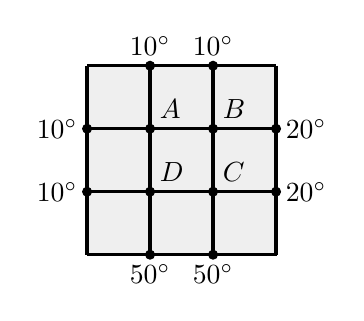
\begin{tikzpicture}[scale=0.8]
      \draw[ultra thin,fill=lightgray!25] (0,0) rectangle (3,-3);

      \draw[-,very thick](0,0)--node[left]{}++(3,0);
      \draw[-,very thick](3,0)--node[left]{}++(0,-3);
      \draw[-,very thick](3,-3)--node[left]{}++(-3,0);
      \draw[-,very thick](0,-3)--node[left]{}++(0,3);
      \draw[-,very thick](1,0)--node[left]{}++(0,-3);
      \draw[-,very thick](2,0)--node[left]{}++(0,-3);
      \draw[-,very thick](0,-1)--node[left]{}++(3,0);
      \draw[-,very thick](0,-2)--node[left]{}++(3,0);

      \filldraw[black] (1,0) circle (2pt) node[above] {$10^\circ$};
      \filldraw[black] (2,0) circle (2pt) node[above] {$10^\circ$};
      \filldraw[black] (0,-1) circle (2pt) node[left] {$10^\circ$};
      \filldraw[black] (0,-2) circle (2pt) node[left] {$10^\circ$};
      \filldraw[black] (1,-3) circle (2pt) node[below] {$50^\circ$};
      \filldraw[black] (2,-3) circle (2pt) node[below] {$50^\circ$};
      \filldraw[black] (3,-1) circle (2pt) node[right] {$20^\circ$};
      \filldraw[black] (3,-2) circle (2pt) node[right] {$20^\circ$};
      \filldraw[black] (1,-1) circle (2pt) node[above right] {$A$};
      \filldraw[black] (2,-1) circle (2pt) node[above right] {$B$};
      \filldraw[black] (2,-2) circle (2pt) node[above right] {$C$};
      \filldraw[black] (1,-2) circle (2pt) node[above right] {$D$};
    \end{tikzpicture}

    \caption{}
    \label{fig:metalplate}
  \end{figure}

  Let $A$, $B$, $C$, and $D$ denote the temperatures of the four interior nodes
  indicated above. The temperature at each node is approximately equal to the
  average temperature of its four adjacent nodes. For example, $A = \sfrac{10 +
  10 + B + D}{4} \implies 20 = 4A - B - D$.

  \begin{enumerate}
    \label{enum:qst_temperature}

    \item Find the system of four linear equations for each of the interior
      nodes.

    \item Solve for the temperatures of $A$, $B$, $C$, and $D$ by solving the
      linear system in part \textbf{1}.
  \end{enumerate}
\end{question}

\begin{solution}
  \label{sol:temperature} $ $

  \begin{enumerate}
    \label{enum:sol_temperature}

    \item The system of four linear equations for each of the interior nodes is
      \begin{alignat*}{5}
        A &= \frac{10 + 10 + B + D}{4} &&\implies 4A = 20 + B + D &&\implies 4A - B - D &&&= 20 \\
        B &= \frac{10 + 20 + C + A}{4} &&\implies 4B = 30 + C + A &&\implies -A + 4B - C &&&=  30 \\
        C &= \frac{B + 20 + 50 + D}{4} &&\implies 4C = B + 70 + D &&\implies -B + 4C - D &&&=  70 \\
        D &= \frac{A + C + 50 + 10}{4} &&\implies 4D = A + C + 60 &&\implies -A - C + 4D &&&=  60
      \end{alignat*}

    \item We can then write the system of equations as an augmented matrix and
      row reduce to find the temperatures of $A$, $B$, $C$, and $D$.
      \[%
        \begin{bNiceArray}{cccc|c}
          4 & -1 & 0 & -1 & 20 \\
          -1 & 4 & -1 & 0 & 70 \\
          0 & -1 & 4 & -1 & 70 \\
          -1 & 0 & -1 & 4 & 60 \\
        \end{bNiceArray}
        \rref
        \begin{bNiceArray}{cccc|c}
          \circled{1} & 0 & 0 & 0 & 16.25 \\
          0 & \circled{1} & 0 & 0 & 18.75 \\
          0 & 0 & \circled{1} & 0 & 28.75 \\
          0 & 0 & 0 & \circled{1} & 26.25 \\
        \end{bNiceArray}
        \longleftrightarrow
        \sysdelim..\systeme{
          A = \SI{16.25}{\degree\fahrenheit},
          B = \SI{18.75}{\degree\fahrenheit},
          C = \SI{28.75}{\degree\fahrenheit},
          D = \SI{26.25}{\degree\fahrenheit}
        }
      .\qedhere\]%
  \end{enumerate}
\end{solution}

% subsection finding_average_temperature (end)

\subsection{Interpolating Polynomial}
\label{sub_sec:interpolating_polynomial}

\begin{question}
  \label{qst:interpolating_polynomial}

  The graph of $y = ax^2 + bx + c$ passes through the points $(2, -8)$, $(-1,
  -2)$, and $(6, -100)$. Note that $a$, $b$, and $c$ are constants.
  \begin{enumerate}
    \label{enum:qst_interpolating_polynomial}

    \item Find a linear system by writing a linear equation for each point.

    \item Find the coefficients a, b, and c by solving the linear system in part
      \textbf{1}.

    \item Using your answers in part \textbf{2}, find the value of $y$ when $x =
      1$. If necessary, round your answer to three decimal places.
  \end{enumerate}
\end{question}

\begin{solution}
  \label{sol:interpolating_polynomial} $ $

  \begin{enumerate}
    \label{enum:sol_interpolating_polynomial}

    \item The linear system is
      \begin{alignat*}{4}
        (2, -8) &\implies -8 &&= a(2)^2 + b(2) + c &&\implies 4a + 2b + c &&= -8 \\
        (-1, -2) &\implies -2 &&= a(-1)^2 + b(-1) + c &&\implies a - b + c &&= -2 \\
        (6, -100) &\implies -100 &&= a(6)^2 + b(6) + c &&\implies 36a + 6b + c &&= -100
      \end{alignat*}

    \item We can then write the system of equations as an augmented matrix and
      row reduce to find the coefficients $a$, $b$, and $c$.
      \[%
        \begin{bNiceArray}{ccc|c}[columns-width=auto]
          4 & 2 & 1 & -8 \\
          1 & -1 & 1 & -2 \\
          36 & 6 & 1 & -100 \\
        \end{bNiceArray}
        \rref
        \begin{bNiceArray}{ccc|c}[columns-width=auto]
          \circled{1} & 0 & 0 & -3 \\
          0 & \circled{1} & 0 & 1 \\
          0 & 0 & \circled{1} & 2 \\
        \end{bNiceArray}
        \longleftrightarrow
        \sysdelim..\systeme*{
          a = -3,
          b = 1,
          c = 2
        }
      .\]%

    \item We can then plug in $a = -3$, $b = 1$, and $c = 2$ into the equation
      $y = ax^2 + bx + c$ to find the value of $y$ when $x = 1$, giving us $y =
      -3(1)^2 + (1) + 2 = 1$.\qedhere
  \end{enumerate}
\end{solution}

\begin{note}
  \label{nte:interpolating_polynomial}

  The polynomial found in the example above is called the \textbf{interpolating
  polynomial} of the given data. The degree of an interpolating polynomial is
  one less than the number of data points.
\end{note}

% subsection interpolating_polynomial (end)

\subsection{Vandermonde Matrix}
\label{sub_sec:vandermonde_matrix}

\begin{question}
  \label{qst:vandermonde_matrix}

  In a wind tunnel experiment, the force on a projectile due to air resistance
  was measured at different velocities shown in the table below

  \begin{figure}[H]
    \centering

    \begin{tabular}{|l|c|c|c|c|c|c|}
      \hline
      Velocity (\SI{100}{\foot\per\second}) & $0$ & $2$ & $4$ & $6$ & $8$ & $10$ \\
      \hline
      Force (\SI{100}{\pound}) & $0$ & $3.35$ & $18.01$ & $37.22$ & $80.31$ & $122.10$ \\
      \hline
    \end{tabular}

    \caption{}
    \label{fig:vandermonde_matrix}
  \end{figure}

  The force F at a specific velocity v can be modeled by the fifth degree
  polynomial
  \[%
    F(v) = a_0 + a_1v + a_2v^2 + a_3v^3 + a_4v^4 + a_5v^5
  ,\]%
  where $a_1$, $a_2$, $a_3$, $a_4$, and $a_5$ are constants.
  \begin{enumerate}
    \label{enum:qst_vandermonde_matrix}

    \item Find a linear system by writing a linear equation for each data point
      in the table above.

    \item Find the coefficients $a_1$, $a_2$, $a_3$, $a_4$, and $a_5$ by solving
      the linear system in part \textbf{1}.

    \item Using your answer in part \textbf{2}, what is the force on the
      projectile when the velocity is \SI{850}{\foot\per\second}?
  \end{enumerate}
\end{question}

\begin{solution}
  \label{sol:vandermonde_matrix} $ $

  \begin{enumerate}
    \label{enum:sol_vandermonde_matrix}

    \item The linear system is
      \begin{alignat*}{4}
        (0, 0) &\implies a_0 + a_1(0) + a_2(0)^2 + a_3(0)^3 + a_4(0)^4 + a_5(0)^5 &&= 0 \\
        (2, 3.35) &\implies a_0 + a_1(2) + a_2(2)^2 + a_3(2)^3 + a_4(2)^4 + a_5(2)^5 &&= 3.35 \\
        (4, 18.01) &\implies a_0 + a_1(4) + a_2(4)^2 + a_3(4)^3 + a_4(4)^4 + a_5(4)^5 &&= 18.01 \\
        (6, 37.22) &\implies a_0 + a_1(6) + a_2(6)^2 + a_3(6)^3 + a_4(6)^4 + a_5(6)^5 &&= 37.22 \\
        (8, 80.31) &\implies a_0 + a_1(8) + a_2(8)^2 + a_3(8)^3 + a_4(8)^4 + a_5(8)^5 &&= 80.31 \\
        (10, 122.10) &\implies a_0 + a_1(10) + a_2(10)^2 + a_3(10)^3 + a_4(10)^4 + a_5(10)^5 &&= 122.10
      \end{alignat*}

    \item We can then write the system of equations as an augmented matrix and
      row reduce to find the coefficients $a_1$, $a_2$, $a_3$, $a_4$, and $a_5$.
      \[%
        \begin{bNiceArray}{cccccc|c}[columns-width=auto]
          1 & 0 & 0 & 0 & 0 & 0 & 0 \\
          1 & 2 & 2^2 & 2^3 & 2^4 & 2^5 & 3.35 \\
          1 & 4 & 4^2 & 4^3 & 4^4 & 4^5 & 18.01 \\
          1 & 6 & 6^2 & 6^3 & 6^4 & 6^5 & 37.22 \\
          1 & 8 & 8^2 & 8^3 & 8^4 & 8^5 & 80.31 \\
          1 & 10 & 10^2 & 10^3 & 10^4 & 10^5 & 3.35 \\
        \end{bNiceArray}
        \rref\hspace{0.3cm}
        \begin{bNiceArray}{ll}[columns-width=auto]
          a_0 \approx & 0 \\
          a_1 \approx & -12.600 \\
          a_2 \approx & 12.602 \\
          a_3 \approx & -3.530 \\
          a_4 \approx & 0.4357 \\
          a_5 \approx & -0.018 \\
        \end{bNiceArray}
      .\]%

    \item We input $v = \sfrac{856}{100} = 8.5$ into $F(v)$
      \[%
        F(8.5) \approx 0 - 12.600(8.5) + 12.602(8.5)^2 - 3.530(8.5)^3 + 0.4357(8.5)^3 + 0.4357(8.5)^4 - 0.0184(8.5)^5 \approx 93.497
      ,\]%
      which is $93.497$ per \SI{100}{\pound}, or \SI{9349.7}{\pound}.\qedhere
  \end{enumerate}
\end{solution}

% subsection projectile_motion (end)

% section vandermonde_matrix (end)

\newpage
